% ============================================================
% 第七章 样机制作与实验验证
% ============================================================

\chapter{样机制作与实验验证}

\section{样机制作过程}

\subsection{3D打印节点制作}

PLA节点结构件采用FDM（熔融沉积成型）工艺打印，
打印设备为拓竹 Bambu Lab P2S，
打印参数如表~\ref{tab:print_params}所示。

\begin{longtable}{ll}
    \caption{PLA节点3D打印参数}
    \label{tab:print_params} \\

    % -------- 第一页表头 --------
    \toprule
    参数 & 设置值 \\
    \midrule
    \endfirsthead

    % -------- 续页表头 --------
    \multicolumn{2}{l}{\small 续表~\ref*{tab:print_params}} \\[2pt]
    \toprule
    参数 & 设置值 \\
    \midrule
    \endhead

    % -------- 每页底部（非末页）--------
    \midrule
    \multicolumn{2}{r}{\small 接下页} \\
    \endfoot

    % -------- 最后一页底部 --------
    \bottomrule
    \endlastfoot

    % -------- 表格内容 --------
    打印设备        & 拓竹 Bambu Lab P2S \\[3pt]
    打印材料        & PLA（拓竹原厂耗材） \\[3pt]
    层高            & 0.20\,mm \\[3pt]
    填充密度        & 15\%（网格填充） \\[3pt]
    壁厚            & 3 圈（约 1.2\,mm） \\[3pt]
    打印温度        & 220\,$^\circ$C \\[3pt]
    热床温度        & 55\,$^\circ$C（PEI板） \\[3pt]
    打印速度        & 200\,mm/s（拓竹P2S标准预设） \\[3pt]
    支撑类型        & 树状支撑（接触间距 0.2\,mm） \\[3pt]
    打印时间（合计）& 约 34\,h \\

\end{longtable}

节点结构件共14件，包括四角电机安装节点、
边框中点连接节点、中心飞控安装平台等，总打印质量约600\,g。
树状支撑在打印完成后可徒手掰除，对节点表面质量影响极小。
旋翼保护圈与角节点结构件经历了多轮设计迭代，
如图~\ref{fig:node_iteration}所示，
从早期轻量化保护圈逐步演进为集成气柱接口、电机安装座与骨架连接件的一体化角节点，
最终版本在结构强度、装配精度与重量控制之间取得了较好的平衡。

\begin{figure}[htbp]
    \centering
    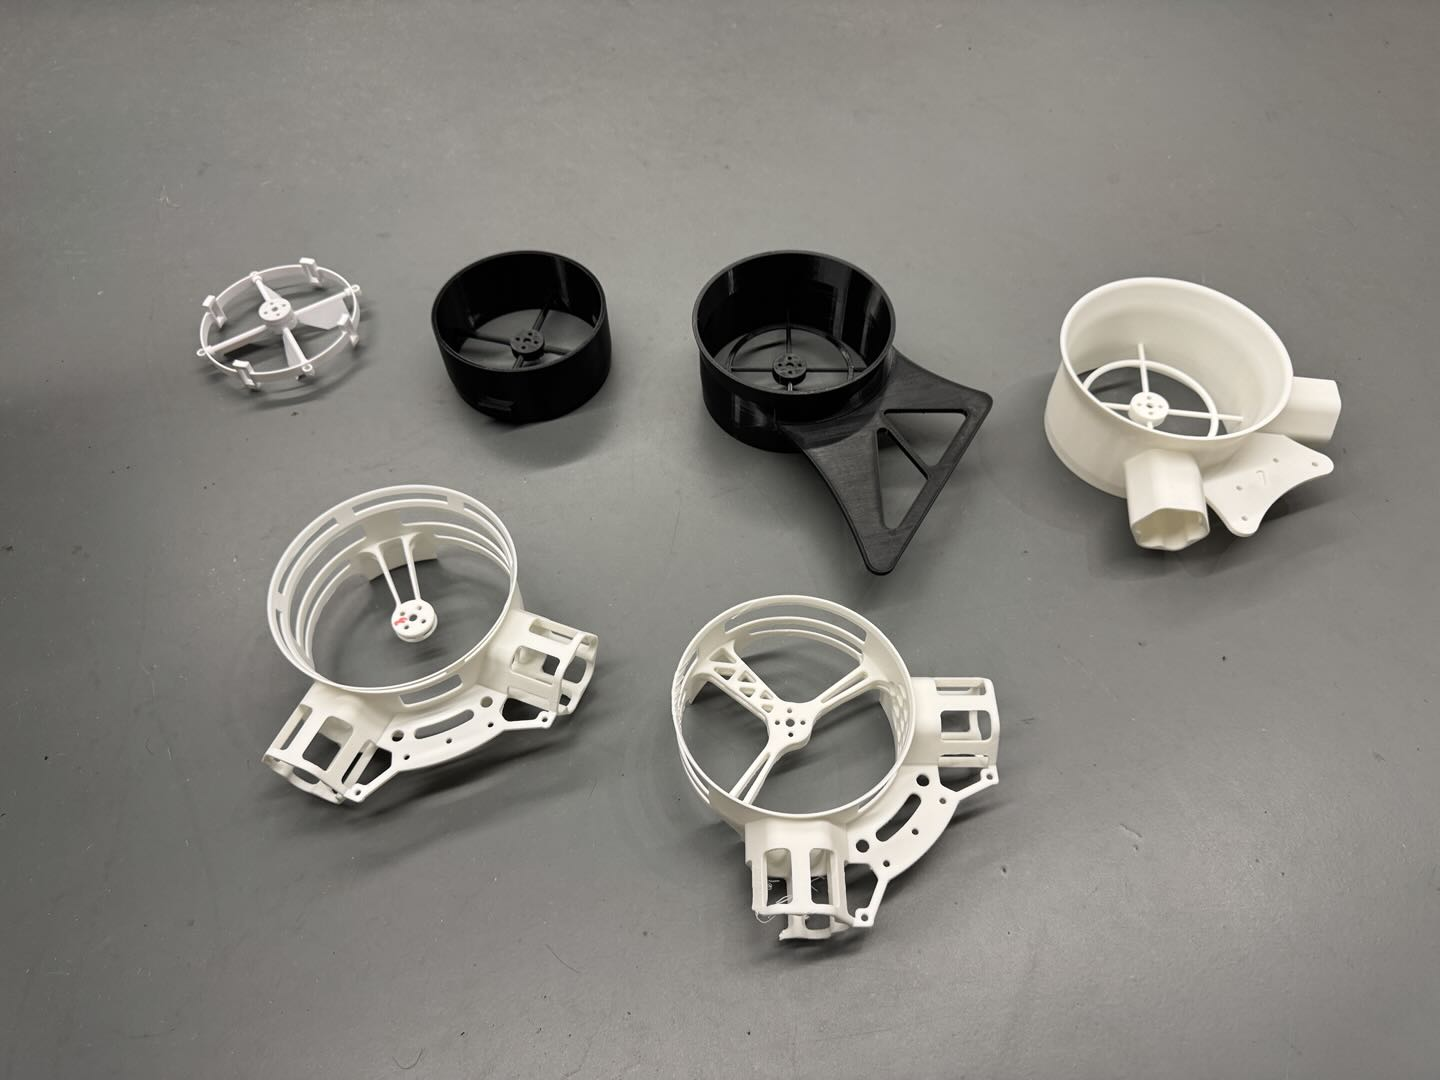
\includegraphics[width=0.75\textwidth]{figures/fig7_node_iteration.jpeg}
    \caption{旋翼保护圈与角节点结构件设计迭代过程（从左至右依次为各代版本）}
    \label{fig:node_iteration}
\end{figure}


\subsection{充气骨架组装}

充气骨架的组装流程如下：

\begin{enumerate}
    \item 将标准快递气柱按设计长度裁切，端部折叠密封；
    \item 将气柱穿入PLA节点接口，用扎带或卡扣固定；
    \item 依次完成四条外框边、四条中心辐射杆的连接；
    \item 安装中心飞控平台，固定伞面固定架；
    \item 充气测试，检验各节点气密性，确认骨架展开形态。
\end{enumerate}


集成完成后整机重量实测为 1683\,g，
较质量预算（1468\,g）偏高约 14.6\%（超出215\,g）。


\subsection{电子系统集成}

电子系统集成按以下步骤完成：

\begin{enumerate}
    \item 四个电机安装于旋翼保护圈内侧电机座，用 M3 螺栓固定；
    \item ESC 沿骨架气柱外侧布线，用扎带固定，三相线与电机焊接；
    \item Pixhawk~6C 安装于中心飞控平台，减震垫隔振；
    \item GPS 模块固定于伞面固定架顶端，磁罗盘朝上；
    \item R9DS 接收机固定于中心平台侧面，天线展开朝向外侧；
    \item 电源分配板（PDB）固定于中心平台下方，连接四个 ESC 与电源接口。
\end{enumerate}

电子系统集成完成后的中心飞控平台实物如图~\ref{fig:electronics}所示，
Pixhawk~6C 飞控安装于顶层，通过减震硅胶垫与中心平台隔振；
PDB 位于中层，四路 ESC 信号线与电源线沿骨架气柱外侧布线引出；
XT60 电源接口朝下引出，便于系留供电缆线的快速插拔。

\begin{figure}[htbp]
    \centering
    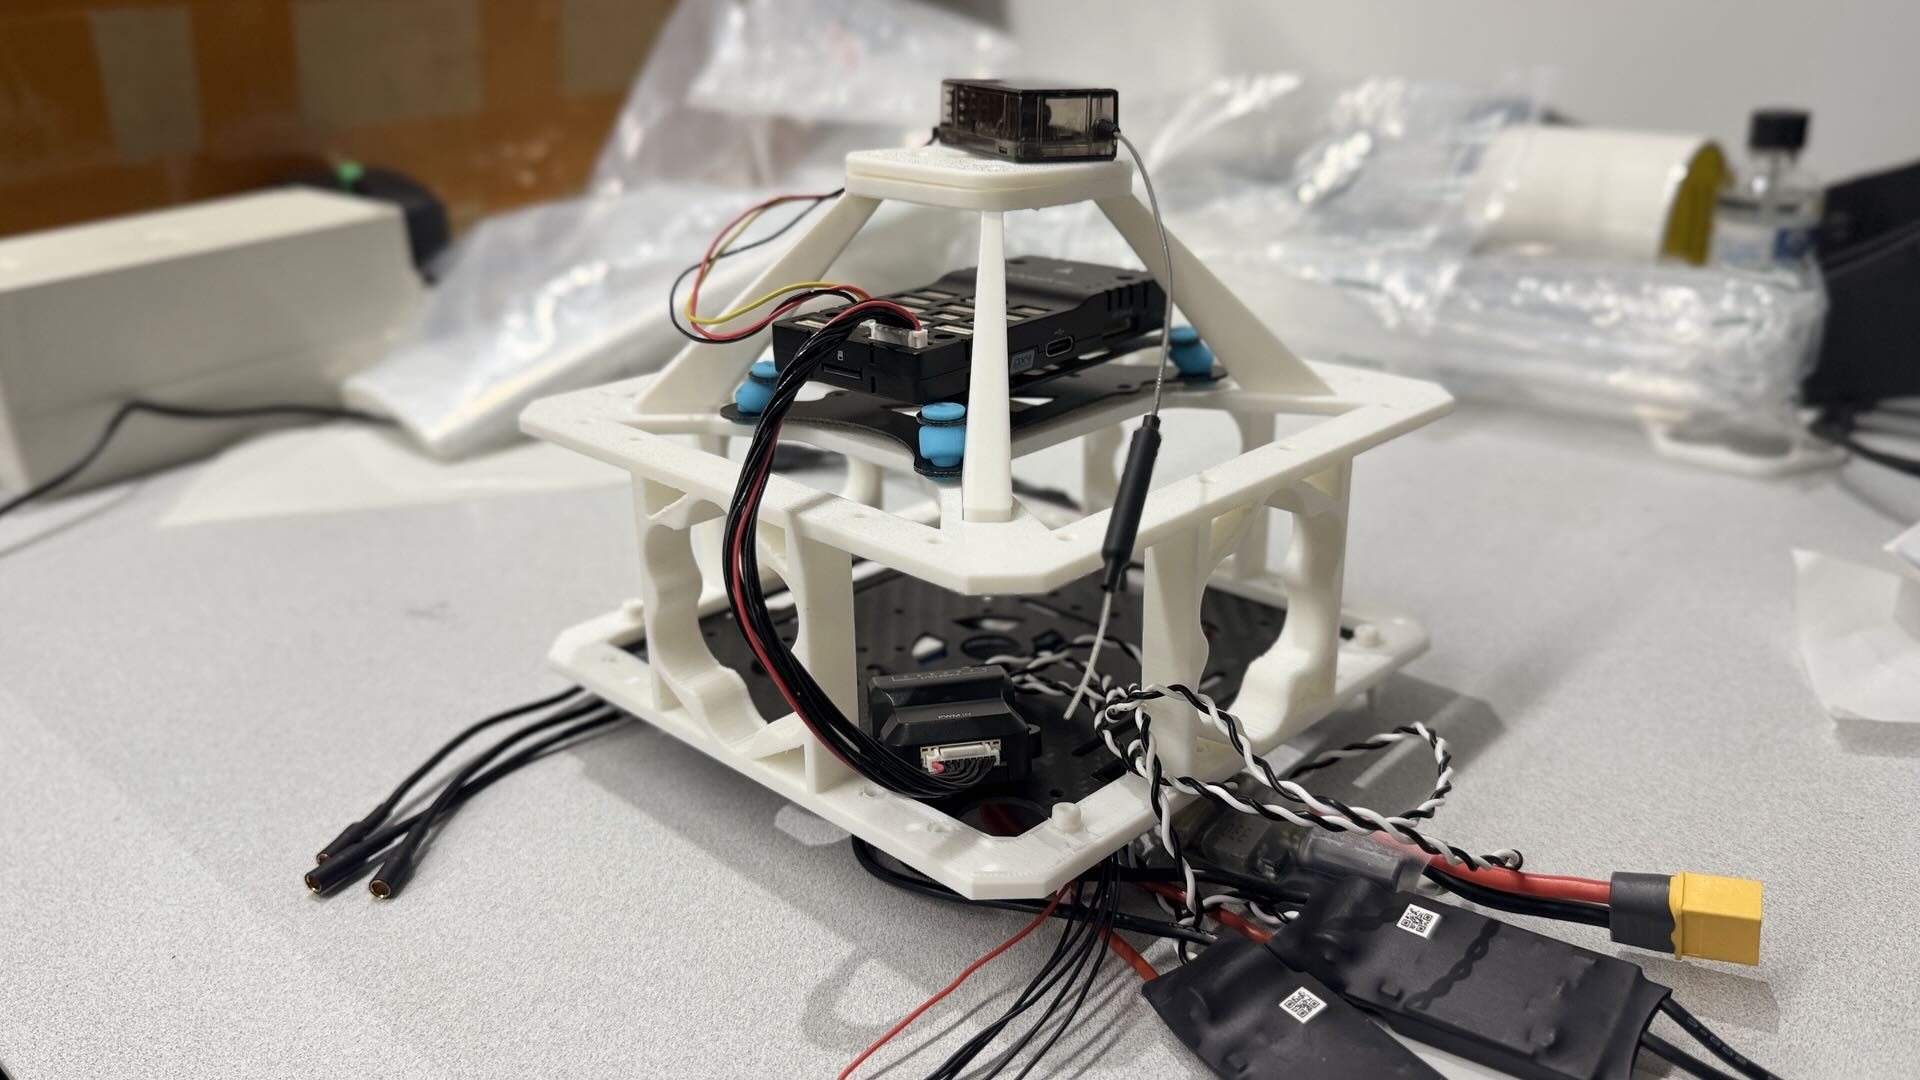
\includegraphics[width=0.75\textwidth]{figures/fig7_electronics.jpeg}
    \caption{电子系统集成完成后的中心飞控平台实物（顶部为 Pixhawk~6C，中层为 PDB，蓝色为减震垫）}
    \label{fig:electronics}
\end{figure}
\FloatBarrier   % ← 新增


整机实测起飞质量 1683\,g，较质量预算（1468\,g）偏高约 14.6\%，
超出部分（215\,g）主要来源于以下几个方面：

\begin{itemize}
    \item PLA 节点结构件实际打印质量高于估算值，
          原因是部分节点在迭代过程中增加了壁厚与填充密度；
    \item 系留缆线（14\,AWG，约 150\,cm）及连接器的实际重量
          未计入原始质量预算；
    \item 气柱骨架固定用的扎带、热熔胶等辅助连接件合计约 30\,g。
\end{itemize}

以实测起飞质量为基准，依据第四章推力数据，
系统在 50\% 油门时四旋翼合计推力约 3400\,gf，
推重比约 $3400/1683 \approx 2.02$，满足设计指标（$\geq 1.5$）；
在 70\% 油门下推重比可达 $4600/1683 \approx 2.73$，
动力裕量足够支撑稳定悬停。
整机集成完成后的充气展开状态如图~\ref{fig:drone_full} 所示，
正方形气柱骨架、四角旋翼单元与中心飞控平台的空间布局
与第三章设计方案基本吻合。

\begin{figure}[htbp]
    \centering
    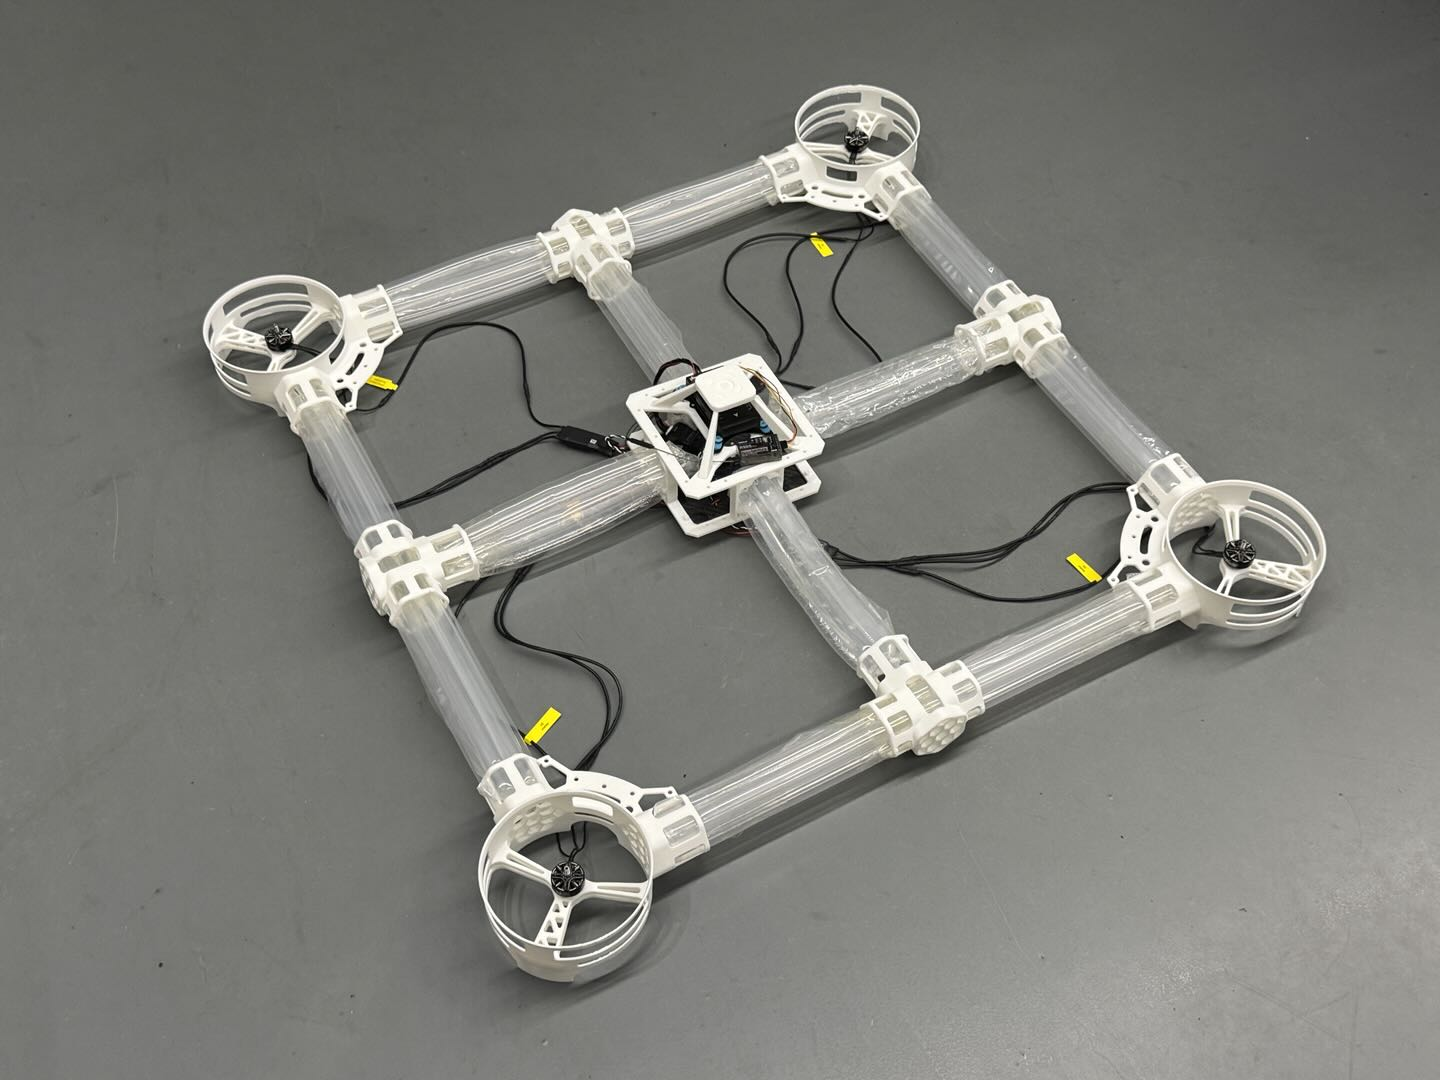
\includegraphics[width=0.75\textwidth]{figures/fig7_drone_full.jpeg}
    \caption{飞行雨伞工程样机整机俯视图（充气展开状态，未安装TPU伞面）}
    \label{fig:drone_full}
\end{figure}
\FloatBarrier 


\section{充气结构性能测试}

\subsection{充气展开时间测试}

使用车载微型充气泵对骨架进行充气，如图~\ref{fig:pump_photo}所示。
\begin{figure}[htbp]
    \centering
    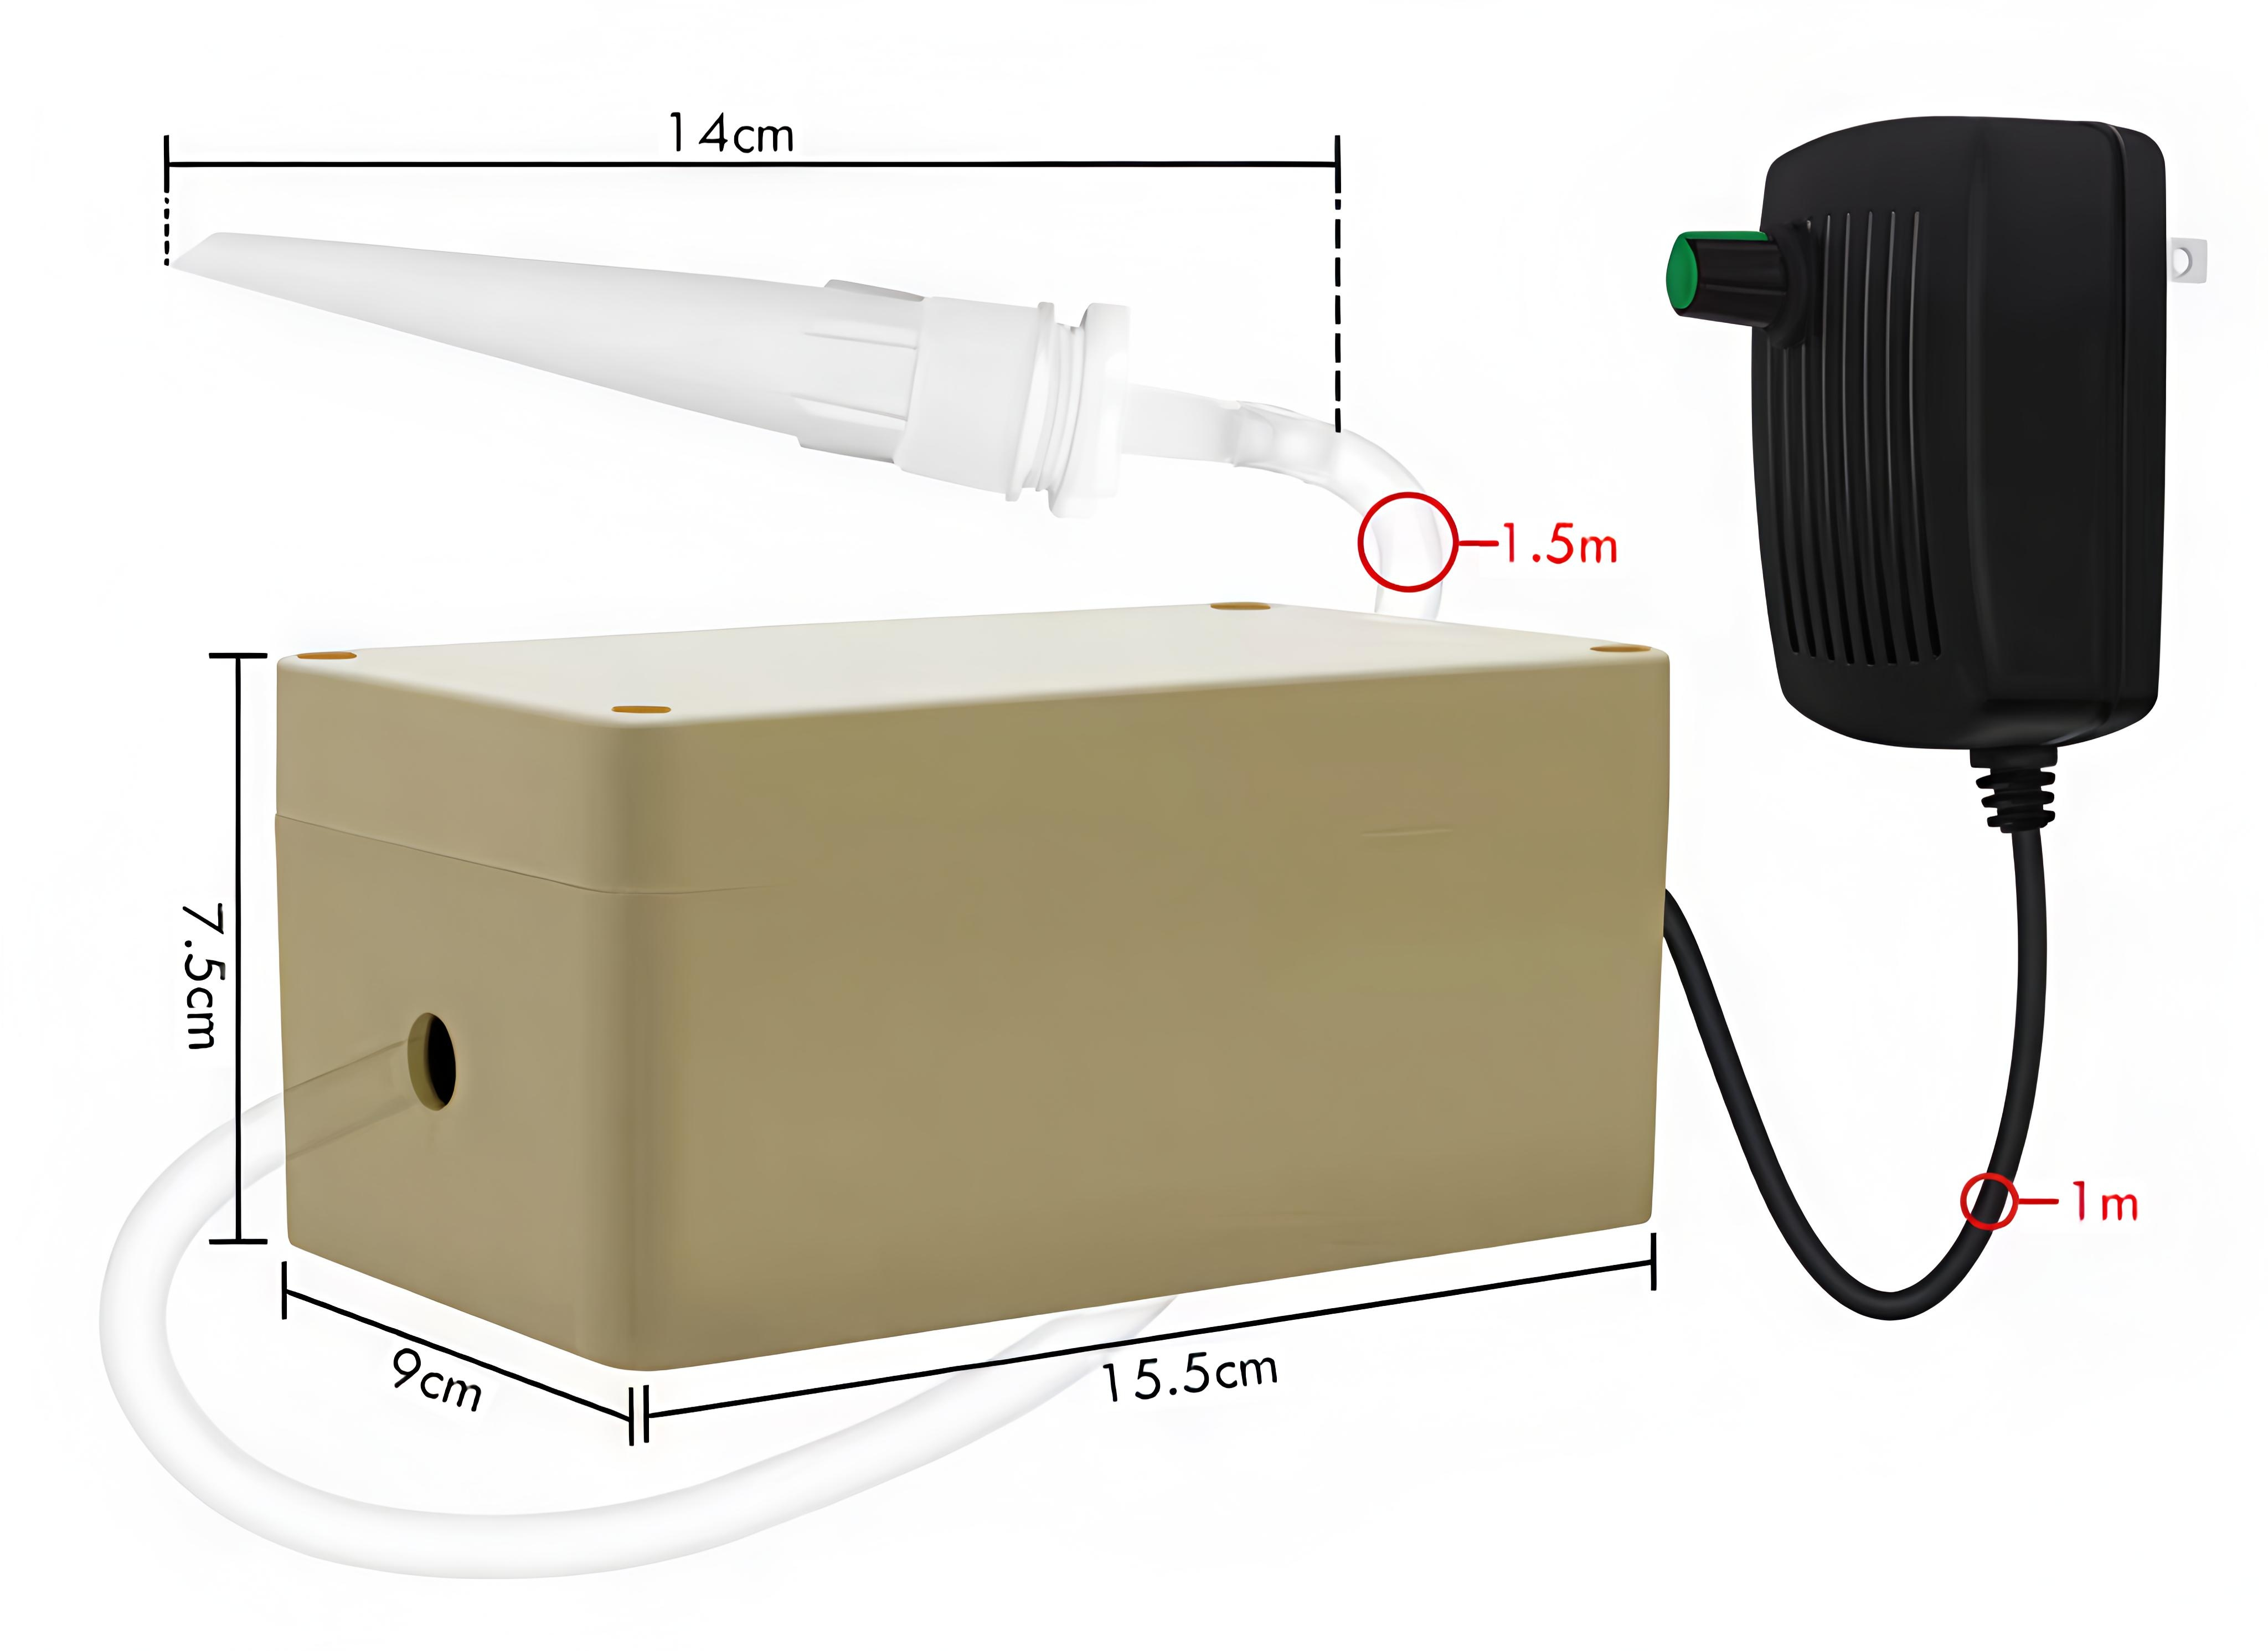
\includegraphics[width=0.45\textwidth]{figures/fig7_pump_photo.png}
    \caption{车载微型充气泵实物图}
    \label{fig:pump_photo}
\end{figure}
\FloatBarrier
计时从开启充气泵到\textbf{单根气柱}完全充气（达到工作气压）所需时间；
整个骨架（含全部气柱）的总充气展开时间见7.4节完整流程验证。
由于本文样机采用的商业快递气柱设有单向止回阀，
正常状态下无法通过气嘴直接排气，
故实际测试时通过刺破气囊模拟快速放气过程。

因此，表~\ref{tab:inflation_test}中的排气收纳时间为基于刺破实验测算的预估值。
重复测试5次，测试结果如下。



\begin{longtable}{lr}
    \caption{充气展开时间测试结果}
    \label{tab:inflation_test} \\

    % -------- 第一页表头 --------
    \toprule
    测试项目 & 结果 \\
    \midrule
    \endfirsthead

    % -------- 续页表头 --------
    \multicolumn{2}{l}{\small 续表~\ref*{tab:inflation_test}} \\[2pt]
    \toprule
    测试项目 & 结果 \\
    \midrule
    \endhead

    % -------- 每页底部（非末页）--------
    \midrule
    \multicolumn{2}{r}{\small 接下页} \\
    \endfoot

    % -------- 最后一页底部（含脚注）--------
    \bottomrule
    \multicolumn{2}{p{10cm}}{%
        \footnotesize $^{*}$ 受限于单向阀结构，此处排气时间为刺破\textbf{单根气柱}后的
        快速放气预估值；完整工作流程中"降落到排气收纳完成"的实测时间为48\,s
        （含降落、拆卸缆线、逐根排气折叠等步骤），见7.4节。} \\
    \endlastfoot

    % -------- 设备参数 --------
    充气泵型号       & 静音气柱充气机 \\[2pt]
    额定流量         & 25\,L/min \\[2pt]
    峰值正压         & $\geq 80$\,kPa \\
    \midrule
    % -------- 充气时间 --------
    平均充气时间     & 43\,s \\[2pt]
    最短充气时间     & 38\,s \\[2pt]
    最长充气时间     & 51\,s \\
    \midrule
    % -------- 排气估值 --------
    排气收纳时间$^{*}$ & $\approx 20$\,s \\

\end{longtable}

\subsection{气密性保持测试}
骨架充气完成后，关闭充气阀，持续观察气柱压力变化，
记录气柱维持有效工作气压的时长，以验证气密性满足使用需求。

测试结果：气柱在充气完成后持续保持工作气压超过30\,min，
满足单次使用时长（约5$\sim$10\,min）的气密性要求。

\section{飞行性能测试}

\subsection{测试环境与条件}

飞行测试在实验室室内场地进行，测试条件如表~\ref{tab:test_condition}所示。

\begin{longtable}{ll}
    \caption{飞行测试环境条件}
    \label{tab:test_condition} \\

    % -------- 第一页表头 --------
    \toprule
    条件项目 & 测试值 \\
    \midrule
    \endfirsthead

    % -------- 续页表头 --------
    \multicolumn{2}{l}{\small 续表~\ref*{tab:test_condition}} \\[2pt]
    \toprule
    条件项目 & 测试值 \\
    \midrule
    \endhead

    % -------- 每页底部（非末页）--------
    \midrule
    \multicolumn{2}{r}{\small 接下页} \\
    \endfoot

    % -------- 最后一页底部 --------
    \bottomrule
    \endlastfoot

    % -------- 表格内容 --------
    测试日期     & 2026年5月6日 \\[3pt]
    测试地点     & 室内实验室 \\[3pt]
    气温         & 约 24\,$^\circ$C \\[3pt]
    风速         & 基本无风（室内环境） \\[3pt]
    供电方式     & 系留供电，6S 10000\,mAh \\[3pt]
    飞行模式     & 姿态稳定模式（Stabilize） \\

\end{longtable}

\subsection{悬停稳定性测试}

\subsubsection{绑绳悬停测试}

首次通电飞行前，采用绑绳约束方式进行安全测试：
用四根长约1\,m的软绳从四角方向固定飞行器，
推油门至悬停点，观察姿态稳定性。

测试结果：按第五章预设参数上电后，Roll轴出现约$\pm4^\circ$的轻微低频震荡，
将 \texttt{MC\_ROLLRATE\_P} 由0.050进一步调低至0.040后震荡消除，
Pitch轴参数同步调整，绑绳状态下姿态稳定，参数调整过程与第五章整定策略一致。

\subsubsection{自由悬停测试}

解除绑绳后进行自由悬停测试，
飞行器在姿态稳定模式下由操作者手动控制悬停于地面以上约2.1\,m处
（受室内场地净高限制，低于设计工作高度上限2.5\,m），
持续飞行时长约5\,min（300\,s）。

主要测试结果如表~\ref{tab:hover_result}所示。

\begin{longtable}{p{4.5cm} p{3.5cm} p{3.5cm}}
    \caption{自由悬停测试结果}
    \label{tab:hover_result} \\

    % -------- 第一页表头 --------
    \toprule
    测试指标 & 测试结果 & 设计目标 \\
    \midrule
    \endfirsthead

    % -------- 续页表头 --------
    \multicolumn{3}{l}{\small 续表~\ref*{tab:hover_result}} \\[2pt]
    \toprule
    测试指标 & 测试结果 & 设计目标 \\
    \midrule
    \endhead

    % -------- 每页底部（非末页）--------
    \midrule
    \multicolumn{3}{r}{\small 接下页} \\
    \endfoot

    % -------- 最后一页底部 --------
    \bottomrule
    \endlastfoot

    % -------- 表格内容 --------
    悬停姿态偏差（Roll）  & $\pm 2.1^\circ$（均值）  & $\leq \pm5^\circ$ \\[3pt]
    悬停姿态偏差（Pitch） & $\pm 1.8^\circ$（均值）  & $\leq \pm5^\circ$ \\[3pt]
    实际悬停油门  & 约 43\%  & 约38\%（整定值） \\[3pt]
    最大飞行高度          & 2.1\,m                   & $\leq 2.5$\,m \\[3pt]
    系留模式续航          & 18.2\,min                & $\geq 15$\,min \\

\end{longtable}

实际悬停油门约 43\%，高于第五章整定的悬停油门预设值（38\%），
原因分析如下：

\begin{enumerate}
    \item \textbf{桨叶效率低于理论值}：
    理论计算中采用品质因数 $\text{FOM} = 0.7$，
    属于高性能桨叶的理想估计。
    实际测试中，51366 MCK v3 桨叶在低转速悬停工况下的气动效率
    低于该值，导致单位油门对应的实际推力偏低。

    \item \textbf{充气伞面附加气动阻力}：
    充气伞面展开后对旋翼下洗流产生侧向扰流，
    维持稳定悬停所需的推力因此有所增加。

    \item \textbf{系留缆线重力分量}：
    系留缆线（约 150\,cm，14\,AWG）自重约 80\,g，
    起飞后缆线悬垂产生向下的附加载荷，
    未计入理论质量预算，使实际起飞质量偏高约 5\%。
\end{enumerate}

虽然实际悬停油门大于设计预估的43\%，但都在电机额定工作范围内
（额定连续油门约 70\%）。
此时推重比约为 1.68（43\% 油门推力 2826\,gf $\div$ 实测质量 1683\,g），
设计指标满足，姿态控制性能没有受到影响。


\subsection{遮雨功能说明}

遮蔽面积方面，第三章已通过几何计算确认伞面展开后的正投影面积为
$0.608\,\text{m}^2$（边长 779.59\,mm 的正方形），
超过设计指标（$\geq 0.40\,\text{m}^2$）约 52\%。
防水性能方面，伞面材料为 TPU（热塑性聚氨酯）薄膜，
充气气压下形成连续无缝的遮护面，对垂直降雨具有阻断能力。
受实验条件限制，本文未在实际降雨环境下开展飞行状态的遮雨功能测试，
该项性能有待后续结合真实降雨场景进行验证。



% ----------------------------------------------------------


\section{完整工作流程验证}

本节对飞行雨伞系统
"收纳$\rightarrow$充气展开$\rightarrow$起飞$\rightarrow$悬停$\rightarrow$降落$\rightarrow$收纳"
完整工作闭环进行计时验证，结果如表~\ref{tab:workflow_result}所示。

\begin{longtable}{p{4.8cm} p{2.8cm} p{3.0cm}}
    \caption{完整工作流程计时验证}
    \label{tab:workflow_result} \\

    % -------- 第一页表头 --------
    \toprule
    流程阶段 & 实测时间 & 设计目标 \\
    \midrule
    \endfirsthead

    % -------- 续页表头 --------
    \multicolumn{3}{l}{\small 续表~\ref*{tab:workflow_result}} \\[2pt]
    \toprule
    流程阶段 & 实测时间 & 设计目标 \\
    \midrule
    \endhead

    % -------- 每页底部（非末页）--------
    \midrule
    \multicolumn{3}{r}{\small 接下页} \\
    \endfoot

    % -------- 最后一页底部 --------
    \bottomrule
    \endlastfoot

    % -------- 表格内容 --------
    取出收纳袋到开始充气  & 13.5\,s  & —            \\[3pt]
    充气展开时间          & 43.0\,s  & $\leq 60$\,s \\[3pt]
    飞控上电到姿态就绪    & 28.5\,s  & —            \\[3pt]
    起飞准备总时间        & 85.0\,s  & $\leq 90$\,s \\[3pt]
    悬停服务时间（本次）  & 300.0\,s & —            \\[3pt]
    降落到排气收纳完成    & 48.0\,s  & $\leq 60$\,s \\

\end{longtable}

\textbf{测试结论：}
完整工作流程顺利完成，充气展开时间 43\,s、起飞准备总时间 85\,s、
排气收纳时间 48\,s，各阶段均达到设计指标。
充气展开与排气收纳操作流程连贯，重复执行结果稳定，
"随车常备、快速部署"的使用方式在工程上可行。


\section{本章小结}

本章记录了飞行雨伞样机的制作过程并完成了实验验证。

样机制作方面，整机实测质量 1683\,g，较质量预算（1468\,g）偏高约 14.6\%，
超出部分主要来源于节点件实际打印质量偏高、系留缆线及辅助连接件未计入预算；
整机质量仍在 $\leq 2.0\,\text{kg}$ 的设计指标范围内。

实验验证方面，充气骨架可持续保持工作气压超过 30\,min；
整骨架充气展开时间 43\,s，起飞准备总时间 85\,s，排气收纳时间 48\,s，
各阶段均达到设计指标（分别为 $\leq$60\,s、$\leq$90\,s、$\leq$60\,s）。
飞行测试中，系统在姿态稳定模式下实现稳定悬停，
Roll 轴偏差 $\pm2.1^\circ$、Pitch 轴偏差 $\pm1.8^\circ$，
均优于 $\leq\pm5^\circ$ 的设计目标；
系留模式续航 18.2\,min，满足 $\geq$15\,min 的指标要求。

实际悬停油门（43\%）高于理论预估（38\%），推重比 1.68，
原因已在 7.3.2 节分析。后续可通过节点件轻量化或桨叶选型优化
进一步降低悬停油门、提升动力裕量。